% Figures mit LateX packages 

%Bar-Chart in Latex
\newcommand{\MetalBarChart}{
{
\begin{center}
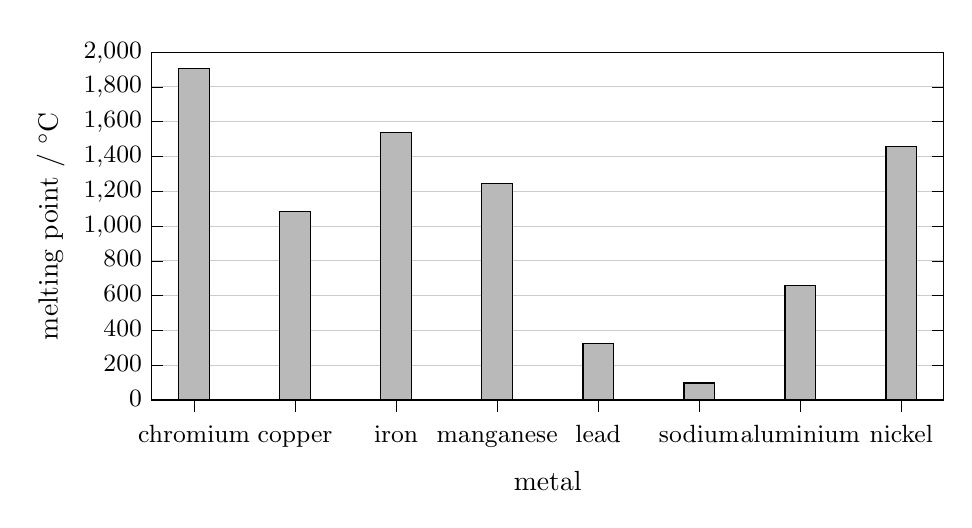
\begin{tikzpicture}
\begin{axis}[
  width=0.96\linewidth,
  height=60mm,
  ybar,
  bar width=11pt,
  ymin=0,
  ymax=2000,
  ylabel={melting point / $^{\circ}$C},
  xlabel={metal},
  symbolic x coords={chromium,copper,iron,manganese,lead,sodium,aluminium,nickel},
  xtick=data,
  typeset ticklabels with strut,
  ytick distance=200,
  ymajorgrids=true,
  grid style={gray!40},
  enlarge x limits=0.06,
  xtick pos=bottom,
  tick style={black},
  x tick label style={font=\small},
  y tick label style={font=\small}
]
\addplot[draw=black, fill=gray!55] coordinates {
  (chromium,1907)
  (copper,1084.62)
  (iron,1538)
  (lead,327.46)
  (manganese,1246)
  (sodium,97.79)
  (aluminium,660.32)
  (nickel,1455)
};
\end{axis}
\end{tikzpicture}
\end{center}
}
}

% Geschwindigkeitsverteilung bei drei Temperaturen
\newcommand{\TempChart}{
{
\begin{center}
	\begin{tikzpicture}
		\begin{axis}[
			width=0.90\linewidth,
			height=65mm,
			xmin=0, xmax=5,
			ymin=0, ymax=0.53,
			axis lines=left,
			xtick=\empty,
			ytick=\empty,
			xlabel={particle speed},
			ylabel={number of particles},
			legend style={
				draw=none,
				fill=none,
				font=\small,
				at={(0.98,0.98)},
				anchor=north east
			},
			samples=130,
			domain=0:5
			]
			
			% Niedrige Temperatur
			\addplot[
			very thick, DeepBlue,
			fill=DeepBlue, fill opacity=0.15
			] {x^2/(0.6^1.5)*exp(-x^2/0.6)} \closedcycle;
			\addlegendentry{Low temperature}
			
			% Mittlere Temperatur
			\addplot[
			very thick, dashed, teal!70!black,
			fill=teal!70!black, fill opacity=0.15
			] {x^2/(1.1^1.5)*exp(-x^2/1.1)} \closedcycle;
			\addlegendentry{Medium temperature}
			
			% Hohe Temperatur
			\addplot[
			very thick, dashdotted, orange!85!black,
			fill=orange!85!black, fill opacity=0.15
			] {x^2/(1.9^1.5)*exp(-x^2/1.9)} \closedcycle;
			\addlegendentry{High temperature}
			
		\end{axis}
	\end{tikzpicture}
\end{center}
}
}

% --- Teilchenbilder fuer homogeneous / heterogeneous mixtures ---

\newcommand{\WideMixtureSketch}[1]{%
	\begin{tikzpicture}[x=1mm,y=1mm]
		\draw[line width=.35mm] (0.25,0) rectangle ++(65,33.5);
		\foreach \j in {0,...,7}{%
			\foreach \i in {0,...,14}{%
				\pgfmathsetmacro{\xx}{3+4.15*\i+mod(\j,2)*1.5}
				\pgfmathsetmacro{\yy}{2.5+4.05*\j}
				\pgfmathtruncatemacro{\kind}{#1}
				\ifcase\kind
				\filldraw[fill=white,draw=black,line width=.2mm] (\xx,\yy) circle (1.8mm);
				\or
				\filldraw[fill=gray!60,draw=black,line width=.2mm] (\xx,\yy) circle (1.8mm);
				\else
				\filldraw[fill=black,draw=black,line width=.2mm] (\xx,\yy) circle (1.8mm);
				\fi
			}%
		}%
	\end{tikzpicture}%
}

% All three particle types are dispersed throughout the mixture.
\newcommand{\HomogeneousMixtureSketch}{%
	\WideMixtureSketch{mod(\i+14*\j,3)}%
}

% Three separate, liquid-like regions; no different densities or particle sizes.
\newcommand{\HeterogeneousMixtureSketch}{%
	\WideMixtureSketch{(\yy<11) ? 0 : ((\yy<19) ? 1 : 2)}%
}
% ============================================================
% Native LaTeX replacements for simple diagrams / worksheets.
% Original image files remain in images/ for reference.
% ============================================================

% Replaces images/scientific_cycle.png and images/brown_cycle.png.
% Unlabelled scientific cycle worksheet: keep the boxes empty.
\newcommand{\ScientificCycleFigure}{%
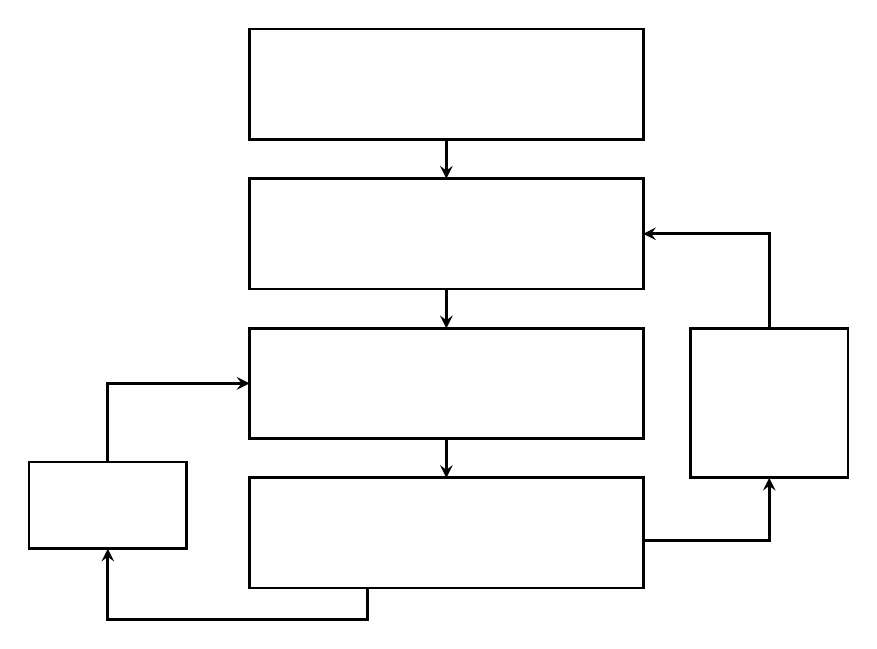
\begin{tikzpicture}[x=1mm,y=1mm,>=stealth,
  box/.style={draw=black,line width=.35mm,fill=white}]
  \draw[box] (-24,67) rectangle (26,81);
  \draw[box] (-24,48) rectangle (26,62);
  \draw[box] (-24,29) rectangle (26,43);
  \draw[box] (-24,10) rectangle (26,24);
  \draw[box] (-52,15) rectangle (-32,26);
  \draw[box] (32,24) rectangle (52,43);
  \draw[->,line width=.35mm] (1,67)--(1,62);
  \draw[->,line width=.35mm] (1,48)--(1,43);
  \draw[->,line width=.35mm] (1,29)--(1,24);
  % Loops from the result back to another step or question.
  \draw[->,line width=.35mm] (-9,10)--(-9,6)--(-42,6)--(-42,15);
  \draw[->,line width=.35mm] (-42,26)--(-42,36)--(-24,36);
  \draw[->,line width=.35mm] (26,16)--(42,16)--(42,24);
  \draw[->,line width=.35mm] (42,43)--(42,55)--(26,55);
\end{tikzpicture}%
}

% Replaces images/image13.png (blank 100 mL graduated cylinder).
\newcommand{\GraduatedCylinderFigure}{%
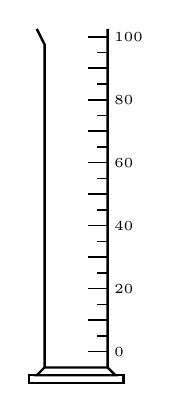
\begin{tikzpicture}[x=1mm,y=1mm,>=stealth]
  \draw[line width=.3mm] (1,47)--(2,45)--(2,4)--(10,4)--(10,47);
  \draw[line width=.3mm] (2,4)--(1,3)--(11,3)--(10,4);
  \draw[line width=.3mm] (0,2) rectangle (12,3);
  \foreach \i in {0,...,20}{%
    \pgfmathsetmacro{\yy}{6+\i*2}
    \draw[line width=.2mm] (10,\yy)--({ifthenelse(mod(\i,2)==0,7.5,8.6)},\yy);
  }
  \foreach \v/\yy in {0/6,20/14,40/22,60/30,80/38,100/46}{%
    \node[font=\tiny,anchor=west,inner sep=0.4mm] at (10.4,\yy) {\v};
  }
\end{tikzpicture}%
}

% Replaces images/image21.png: empty state-of-matter boxes and arrows.
\newcommand{\StateChangesWorksheetFigure}{%
	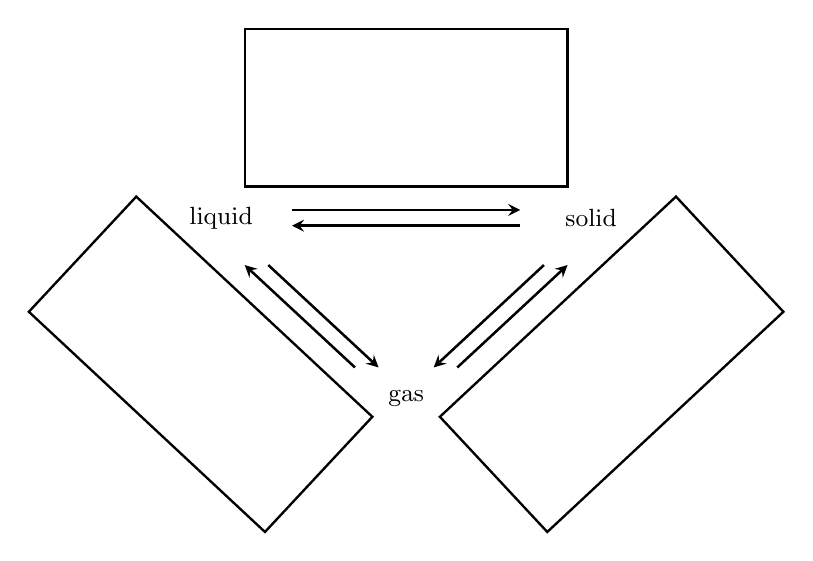
\begin{tikzpicture}[x=1mm,y=1mm,>=stealth,
		every node/.style={font=\small}]
		
		% Top rectangle
		\draw[line width=.3mm]
		(37,35) rectangle (78,55);
		
		% Left rectangle: parallel to liquid-gas arrows
		\begin{scope}[shift={(31.4,12.4)},rotate=-43]
			\draw[line width=.3mm]
			(-20.5,-10) rectangle (20.5,10);
		\end{scope}
		
		% Right rectangle: parallel to solid-gas arrows
		\begin{scope}[shift={(83.6,12.4)},rotate=43]
			\draw[line width=.3mm]
			(-20.5,-10) rectangle (20.5,10);
		\end{scope}
		
		% States of matter
		\node at (34,31) {liquid};
		\node at (81,31) {solid};
		\node at (57.5,8) {gas};
		
		% Liquid <-> Solid
		\draw[->,line width=.32mm] (43,32)--(72,32);
		\draw[->,line width=.32mm] (72,30)--(43,30);
		
		% Liquid <-> Gas
		\draw[->,line width=.32mm] (40,25)--(54,12);
		\draw[->,line width=.32mm] (51,12)--(37,25);
		
		% Solid <-> Gas
		\draw[->,line width=.32mm] (75,25)--(61,12);
		\draw[->,line width=.32mm] (64,12)--(78,25);
		
	\end{tikzpicture}%
}

% Replaces images/diffusion_diagram.png (two boxes and an arrow).
\newcommand{\DiffusionWorksheetFigure}{%
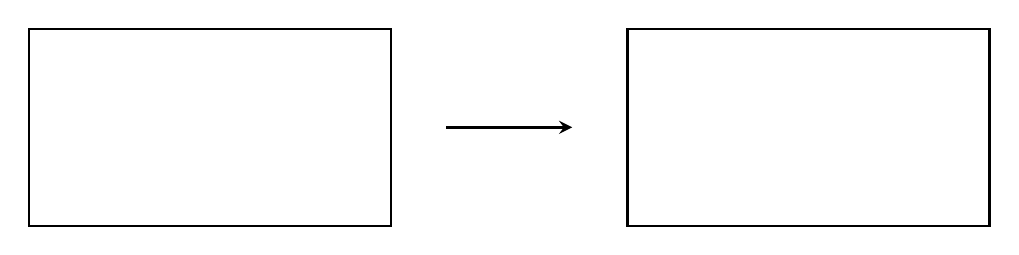
\begin{tikzpicture}[x=1mm,y=1mm,>=stealth]
  \draw[line width=.32mm] (0,0) rectangle (46,25);
  \draw[line width=.32mm] (76,0) rectangle (122,25);
  \draw[->,line width=.38mm] (53,12.5)--(69,12.5);
\end{tikzpicture}%
}

% Replaces images/mixtures_ex20.png (four labelled blank drawing spaces).
\newcommand{\MixtureDrawingWorksheetFigure}{%
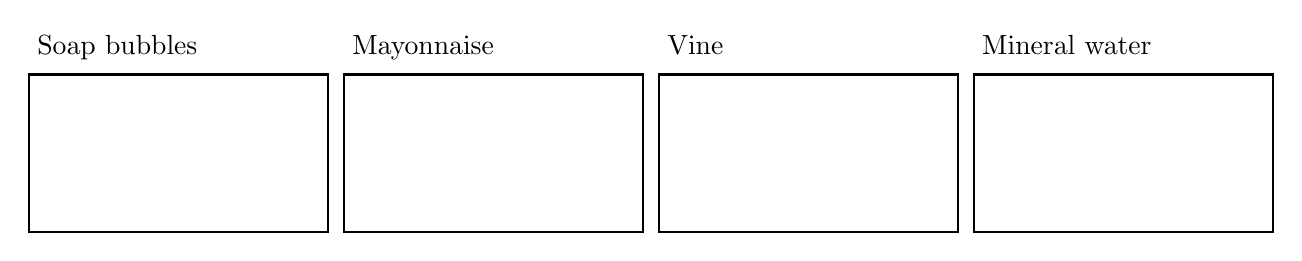
\begin{tikzpicture}[x=1mm,y=1mm]
  \foreach \n/\label in {0/Soap bubbles,1/Mayonnaise,2/Vine,3/Mineral water}{%
    \draw[line width=.32mm] ({40*\n},0) rectangle ({38+40*(\n)},20);
    \node[anchor=north west,inner sep=1mm]
      at ({40*\n},26) {\label};
  }
\end{tikzpicture}%
}

% Replaces images/image43.jpeg (pure substance / element / compound).
\newcommand{\PureSubstanceClassificationFigure}{%
	\resizebox{\linewidth}{!}{%
		\begin{tikzpicture}[x=1mm,y=1mm,>=stealth,
			head/.style={
				draw=DeepBlue,
				rounded corners=1.5mm,
				thick,
				fill=InfoBlue,
				align=center,
				font=\bfseries\small,
				minimum width=36mm,
				minimum height=10mm
			},
			qbox/.style={
				draw=DeepBlue,
				rounded corners=1.5mm,
				thick,
				fill=white,
				align=center,
				font=\small,
				minimum width=42mm,
				minimum height=11mm
			}
			]
			
			% Top level
			\node[head] (sub) at (85,72) {Substances};
			
			% First decision
			\node[qbox] (phys) at (85,54)
			{Separable by physical means?};
			
			% Second level
			\node[head] (pure) at (35,34) {Pure substance};
			\node[head] (mix)  at (135,34) {Mixture};
			
			% Pure substance decision
			\node[qbox] (chem) at (35,16)
			{Separable into simpler\\substances?};
			
			% Mixture decision
			\node[qbox] (uniform) at (135,16)
			{Uniform composition?};
			
			% Final classes
			\node[head] (elem) at (10,-6) {Element};
			\node[head] (comp) at (60,-6) {Compound};
			\node[head] (hetero) at (110,-6) {Heterogeneous\\mixture};
			\node[head] (homo) at (160,-6) {Homogeneous\\mixture};
			
			% Connections top
			\draw[-,thick] (sub.south) -- (phys.north);
			
			\draw[->,thick] (phys.west) -- (35,54) -- (pure.north);
			\draw[->,thick] (phys.east) -- (135,54) -- (mix.north);
			
			\node[font=\small,fill=white,inner sep=1pt] at (52,51) {No};
			\node[font=\small,fill=white,inner sep=1pt] at (118,51) {Yes};
			
			% Pure branch
			\draw[-,thick] (pure.south) -- (chem.north);
			\draw[->,thick] (chem.west) -- (10,16) -- (elem.north);
			\draw[->,thick] (chem.east) -- (60,16) -- (comp.north);
			
			\node[font=\small,fill=white,inner sep=1pt] at (7,13) {No};
			\node[font=\small,fill=white,inner sep=1pt] at (64,13) {Yes};
			
			% Mixture branch
			\draw[-,thick] (mix.south) -- (uniform.north);
			\draw[->,thick] (uniform.west) -- (110,16) -- (hetero.north);
			\draw[->,thick] (uniform.east) -- (160,16) -- (homo.north);
			
			\node[font=\small,fill=white,inner sep=1pt] at (107,13) {No};
			\node[font=\small,fill=white,inner sep=1pt] at (164,13) {Yes};
			
		\end{tikzpicture}%
	}%
}

% Replaces images/physical_summary.png.
\newcommand{\PhysicalProcessSummaryFigure}{%
\begin{tikzpicture}[x=1mm,y=1mm,>=stealth]
  \foreach \x/\y in {2/5,9/13,21/19,8/23,26/8,18/4}{\draw[line width=.25mm] (\x,\y) rectangle ++(3.5,3.5);}
  \foreach \x/\y in {55/7,47/18,45/10,57/21}{\draw[line width=.25mm] (\x,\y)--++(4,0)--++(-2,4)--cycle;}
  \node at (36,14) {$+$};
  \draw[->,thick] (68,16)--(89,16);
  \draw[->,thick] (89,12)--(68,12);
  \foreach \x/\y in {101/19,109/11,102/4,124/0,133/20,136/11}{\draw[line width=.25mm] (\x,\y) rectangle ++(3.5,3.5);}
  \foreach \x/\y in {116/21,126/13,141/3,117/3}{\draw[line width=.25mm] (\x,\y)--++(4,0)--++(-2,4)--cycle;}
\end{tikzpicture}%
}

% Replaces images/chemical_summary.png: differently shaped new products.
\newcommand{\ChemicalReactionSummaryFigure}{%
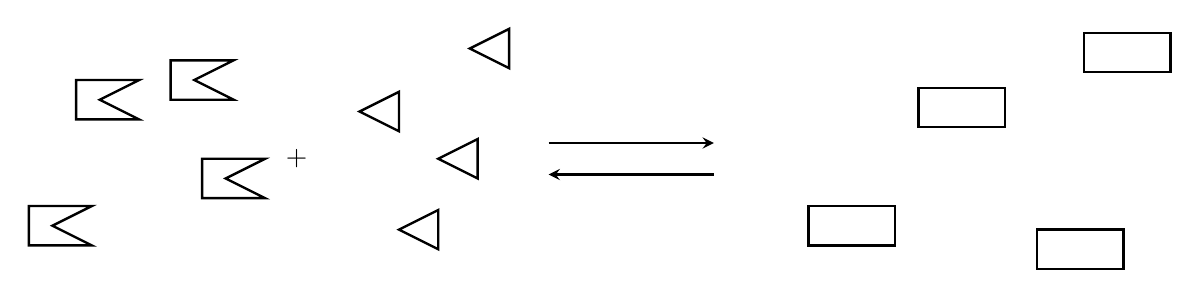
\begin{tikzpicture}[x=1mm,y=1mm,>=stealth]
  \foreach \x/\y in {2/3,8/19,24/9,20/21.5}{%
    \draw[line width=.3mm] (\x,\y)--++(8,0)--++(-5,2.5)--++(5,2.5)--++(-8,0)--cycle;
  }
  \foreach \x/\y in {49/5,44/20,58/28,54/14}{\draw[line width=.3mm] (\x,\y)--++(5,-2.5)--++(0,5)--cycle;}
  \node at (36,14) {$+$};
  \draw[->,thick] (68,16)--(89,16);
  \draw[->,thick] (89,12)--(68,12);
  \foreach \x/\y in {101/3,115/18,136/25,130/0}{\draw[line width=.3mm] (\x,\y) rectangle ++(11,5);}
\end{tikzpicture}%
}

% Replaces images/filtration_diagram.png (submicroscopic / macroscopic).
\newcommand{\FiltrationFigure}{%
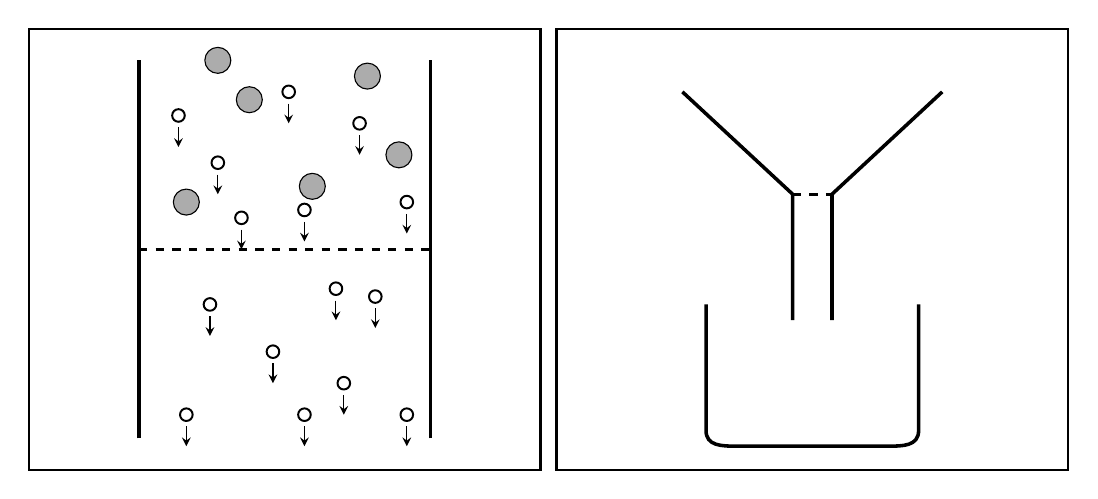
\begin{tikzpicture}[x=1mm,y=1mm,>=stealth]
  \draw[line width=.3mm] (0,0) rectangle (65,56);
  \draw[line width=.3mm] (67,0) rectangle (132,56);
  % Particle-level filtering: solvent through filter, larger solid particles above.
  \draw[line width=.45mm] (14,4)--(14,52) (51,4)--(51,52);
  \draw[very thick,dashed] (14,28)--(51,28);
  \foreach \x/\y in {20/34,28/47,36/36,43/50,47/40,24/52}{%
    \filldraw[fill=gray!65,draw=black] (\x,\y) circle (1.65mm);
  }
  \foreach \x/\y in {19/45,24/39,33/48,42/44,48/34,23/21,31/15,39/23,40/11,20/7,48/7,35/7,27/32,35/33,44/22}{%
    \draw[line width=.25mm,fill=white] (\x,\y) circle (0.8mm);
    \draw[->,thin] (\x,\y-1.5)--(\x,\y-4);
  }
  % Macroscopic set-up: funnel, stem and collecting beaker.
  \draw[line width=.45mm] (83,48)--(97,35)--(97,19);
  \draw[line width=.45mm] (116,48)--(102,35)--(102,19);
  \draw[very thick,dashed] (97,35)--(102,35);
  \draw[line width=.45mm] (86,21)--(86,5) .. controls (86,3) and (88,3) .. (90,3)--(109,3) .. controls (111,3) and (113,3) .. (113,5)--(113,21);
\end{tikzpicture}%
}

% Replaces images/image20.jpg (gas bubbles in a liquid).
% Grey = liquid, closely packed but slightly irregular; white = gas, far apart.
\newcommand{\GasBubblesInLiquidFigure}{%
	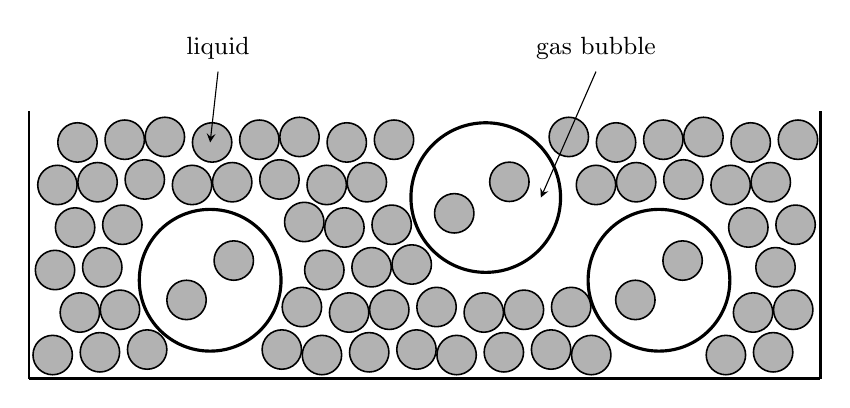
\begin{tikzpicture}[x=1mm,y=1mm,>=stealth]
		\draw[line width=.35mm] (0,0)--(0,34) (100.5,0)--(100.5,34) (0,0)--(100.5,0);
		% Use the *actual* centres/radii of the bubbles when leaving liquid out.
		\foreach \j in {0,...,5}{%
			\foreach \i in {0,...,16}{%
				\pgfmathsetmacro{\px}{3+5.7*\i+2.85*mod(\j,2)+0.30*mod(7*\i+11*\j,3)}
				\pgfmathsetmacro{\py}{3+5.4*\j+0.35*mod(13*\i+3*\j,3)}
				% Add the liquid-particle radius as a safety margin.
				\pgfmathtruncatemacro{\blocked}{%
					((\px-23)^2+(\py-12.5)^2<11.5^2) ||
					((\px-58)^2+(\py-23)^2<12^2) ||
					((\px-80)^2+(\py-12.5)^2<11.5^2)}
				\ifnum\blocked=0
				\filldraw[fill=gray!60,draw=black,line width=.2mm] (\px,\py) circle (2.5mm);
				\fi
			}%
		}%
		\draw[line width=.4mm] (23,12.5) circle[radius=9mm];
		\draw[line width=.4mm] (58,23) circle[radius=9.5mm];
		\draw[line width=.4mm] (80,12.5) circle[radius=9mm];
		\foreach \x/\y in {20/10,26/15,54/21,61/25,77/10,83/15}{%
			\filldraw[fill=gray!60,draw=black,line width=.2mm] (\x,\y) circle (2.5mm);
		}%
		\node[font=\small] at (24,42) {liquid};
		\node[font=\small] at (72,42) {gas bubble};
		\draw[->] (24,39)--(23,30);
		\draw[->] (72,39)--(65,23);
	\end{tikzpicture}%
}

% Replaces images/image16.jpeg (Brownian motion due to random collisions).
\newcommand{\BrownianCollisionFigure}{%
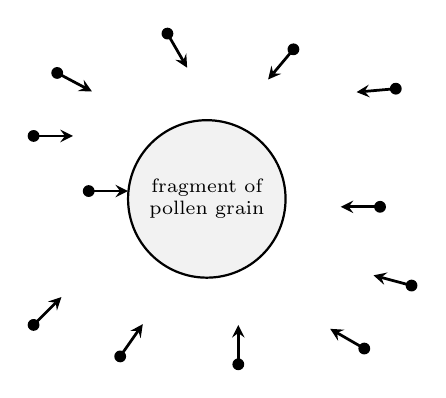
\begin{tikzpicture}[x=1mm,y=1mm,>=stealth]
  \draw[thick,fill=gray!10] (26,24) circle (10mm);
  \node[font=\scriptsize,align=center,text width=17mm]
      at (26,24) {fragment of\\pollen grain};
  \foreach \x/\y/\a in
    {4/8/45,11/25/0,7/40/-28,21/45/-60,37/43/-130,
      50/38/185,48/23/180,46/5/150,30/3/90,15/4/55,
      4/32/0,52/13/165}{%
    \fill (\x,\y) circle (0.75mm);
    \draw[->,line width=.35mm] (\x,\y)--++(\a:5mm);
  }
\end{tikzpicture}%
}

% Replaces images/image17.jpeg (surface reaction of two solids).
% White A-particles and grey B-particles; black C-particles are the products.
\newcommand{\SolidSurfaceReactionFigure}{%
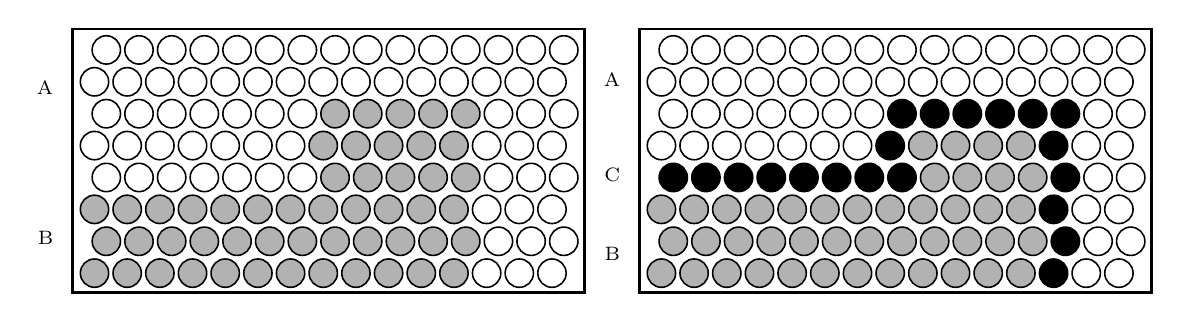
\begin{tikzpicture}[x=1mm,y=1mm,>=stealth]
  \foreach \p in {0,1}{%
    \pgfmathsetmacro{\xshift}{72*\p}
    \draw[line width=.35mm] (\xshift+0.25,0) rectangle ++(65,33.5);
    \foreach \j in {0,...,7}{%
      \foreach \i in {0,...,14}{%
        \pgfmathsetmacro{\xx}{\xshift+3+4.15*\i+mod(\j,2)*1.5}
        \pgfmathsetmacro{\yy}{2.5+4.05*\j}
        \pgfmathtruncatemacro{\isB}{(\i<8 && \j<3) || (\i>6 && \j<6 && \i<12)}
        \pgfmathtruncatemacro{\isC}{\p==1 && ((\i<=7 && \j==3) || (\i==12 && \j<=5) || (\i==7 && \j>=4 && \j<=5) || (\i>=7 && \i<=12 && \j== 5))}
        \ifnum\isC=1
          \filldraw[fill=black,draw=black,line width=.2mm] (\xx,\yy) circle (1.8mm);
        \else
          \ifnum\isB=1
            \filldraw[fill=gray!60,draw=black,line width=.2mm] (\xx,\yy) circle (1.8mm);
          \else
            \filldraw[fill=white,draw=black,line width=.2mm] (\xx,\yy) circle (1.8mm);
          \fi
        \fi
      }
    }
  }
  \node[font=\scriptsize,anchor=east] at (-1,26) {A};
  \node[font=\scriptsize,anchor=east] at (-1,7) {B};
  \node[font=\scriptsize,anchor=east] at (71,27) {A};
  \node[font=\scriptsize,anchor=east] at (71,15) {C};
  \node[font=\scriptsize,anchor=east] at (71,5) {B};
\end{tikzpicture}%
}

% Three car models
% Original image: images/three-car-models.png

\newcommand{\CarModelPanel}[2]{%
	\begin{minipage}[c]{0.314\linewidth}
		\centering
		\fbox{%
			\begin{minipage}[c][33mm][c]{%
					\dimexpr\linewidth-2\fboxsep-2\fboxrule\relax}
				\centering
				\includegraphics[
				width=\linewidth,
				height=31mm,
				keepaspectratio,
				trim={#1bp 11bp #2bp 11bp},
				clip
				]{images/three-car-models.png}
			\end{minipage}%
		}%
	\end{minipage}%
}

\newcommand{\CarModelsFigure}{%
	\begin{center}
		\CarModelPanel{12}{602}\hfill
		\CarModelPanel{294}{328}\hfill
		\CarModelPanel{567}{15}
	\end{center}%
}

% Solubility Curves
% Replaces images/image22.png
% Data points approximated from the original figure.

\newcommand{\SolubilityCurvesFigure}{%
	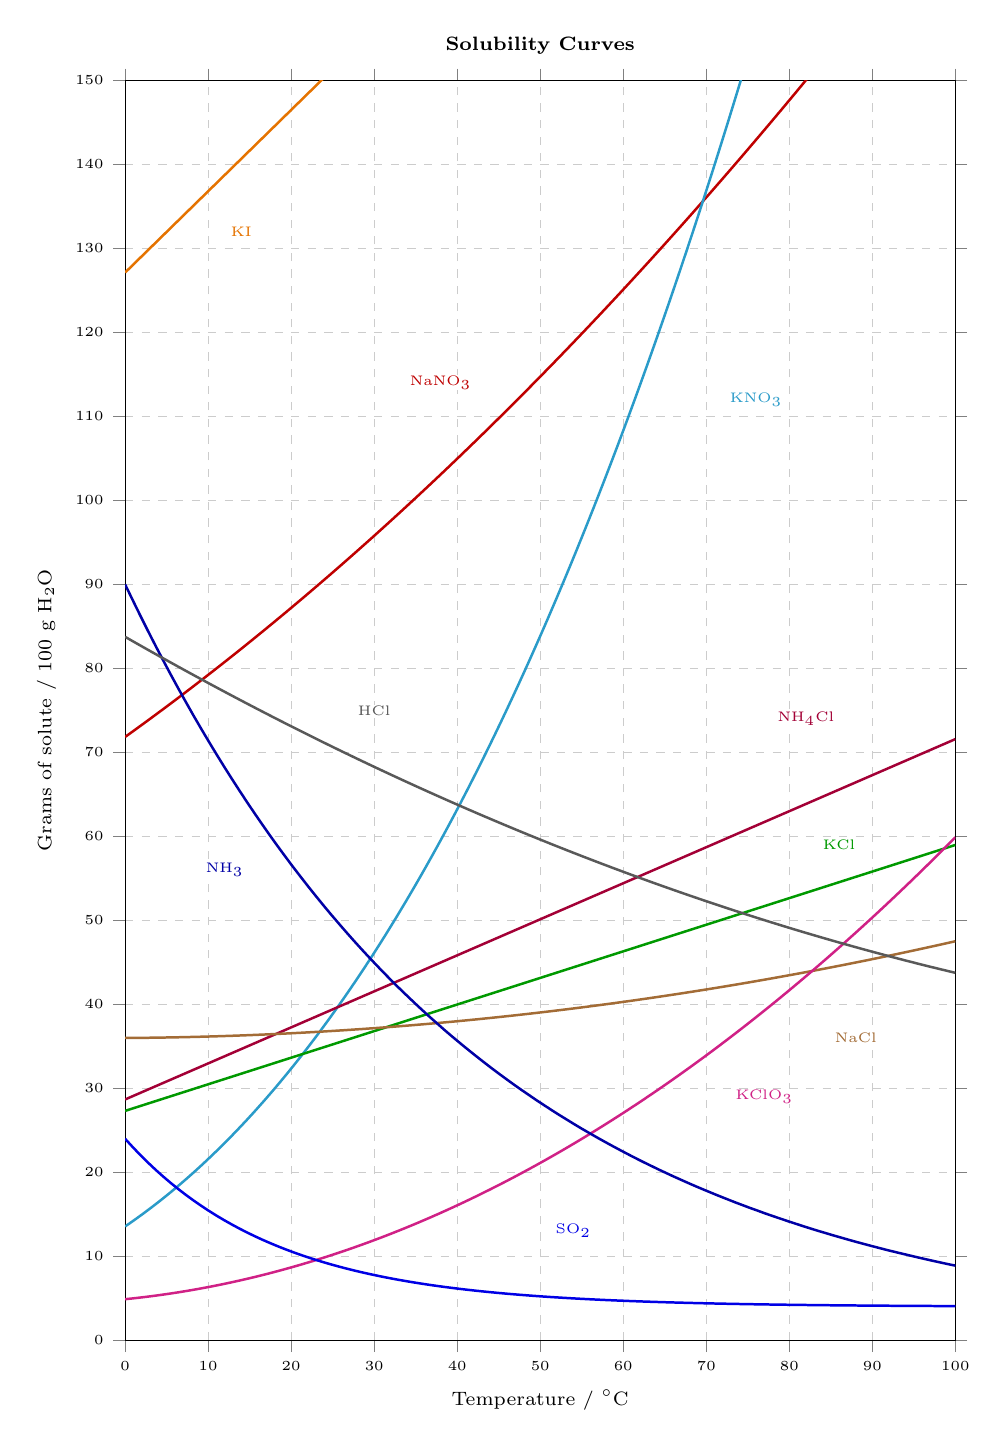
\begin{tikzpicture}
		\begin{axis}[
			width=\linewidth,
			height=1.45\linewidth,
			title={Solubility Curves},
			title style={font=\scriptsize\bfseries},
			xmin=0, xmax=100,
			ymin=0, ymax=150,
			xtick={0,10,...,100},
			ytick={0,10,...,150},
			xmajorgrids=true,
			ymajorgrids=true,
			grid style={gray!40,dashed},
			axis lines=box,
			tick align=outside,
			tick label style={font=\tiny},
			label style={font=\scriptsize},
			xlabel={Temperature / $^\circ$C},
			ylabel={Grams of solute / 100 g H$_2$O},
			every axis plot/.append style={
				mark=none,
				line width=0.9pt,
				samples=110
			},
			clip=true
			]
			
			% Potassium iodide (KI)
			\addplot[orange!90!black, domain=0:26]
			{127.13 + x*(0.96808)};
			
			% Sodium nitrate (NaNO3)
			\addplot[red!75!black, domain=0:84]
			{71.84 + x*(0.70881 + 0.002984*x)};
			
			% Potassium nitrate (KNO3)
			\addplot[cyan!80!black, domain=0:76]
			{13.56 + x*(0.67378 + x*(0.012395 + 0.00004494*x))};
			
			% Ammonium chloride (NH4Cl)
			\addplot[purple!85!black, domain=0:100]
			{28.68 + x*(0.42902)};
			
			% Potassium chloride (KCl)
			\addplot[green!60!black, domain=0:100]
			{27.32 + x*(0.31661)};
			
			% Sodium chloride (NaCl)
			\addplot[brown!85!black, domain=0:100]
			{36 + x*(0.00636 + x*(0.001088))};
			
			% Potassium chlorate (KClO3)
			\addplot[magenta!85!black, domain=0:100]
			{4.90 + x*(0.09895 + 0.0045105*x)};
			
			% Ammonia (NH3)
			\addplot[blue!65!black, domain=0:100]
			{90*exp(-0.02314*x)};
			
			% Hydrogen chloride (HCl)
			\addplot[gray!70!black, domain=0:100]
			{83.76 + x*(-0.5655 + 0.001655*x)};
			
			% Sulphur dioxide (SO2)
			\addplot[blue!90!black, domain=0:100]
			{4 + 20*exp(-x/18)};
			
			% Labels inside the graph
			\node[font=\tiny,text=orange!90!black,fill=white,
			inner sep=0.3pt] at (axis cs:14,132) {KI};
			
			\node[font=\tiny,text=red!75!black,fill=white,
			inner sep=0.3pt] at (axis cs:38,114) {NaNO$_3$};
			
			\node[font=\tiny,text=cyan!80!black,fill=white,
			inner sep=0.3pt] at (axis cs:76,112) {KNO$_3$};
			
			\node[font=\tiny,text=purple!85!black,fill=white,
			inner sep=0.3pt] at (axis cs:82,74) {NH$_4$Cl};
			
			\node[font=\tiny,text=green!60!black,fill=white,
			inner sep=0.3pt] at (axis cs:86,59) {KCl};
			
			\node[font=\tiny,text=brown!85!black,fill=white,
			inner sep=0.3pt] at (axis cs:88,36) {NaCl};
			
			\node[font=\tiny,text=magenta!85!black,fill=white,
			inner sep=0.3pt] at (axis cs:77,29) {KClO$_3$};
			
			\node[font=\tiny,text=blue!65!black,fill=white,
			inner sep=0.3pt] at (axis cs:12,56) {NH$_3$};
			
			\node[font=\tiny,text=gray!70!black,fill=white,
			inner sep=0.3pt] at (axis cs:30,75) {HCl};
			
			\node[font=\tiny,text=blue!90!black,fill=white,
			inner sep=0.3pt] at (axis cs:54,13) {SO$_2$};
			
		\end{axis}
	\end{tikzpicture}%
}

% ------------------------------------------------------------
% Particle-model mixture types for Exercise 1-27.
% Two particle types ONLY, as requested. The state is shown by spacing:
% solid = regular close packing; liquid = disordered close packing;
% gas = widely spaced particles. Same grey/white palette as above.
% ------------------------------------------------------------
\tikzset{
	mixA/.style={draw=black, fill=white},
	mixB/.style={draw=black, fill=gray!60}
}

\newcommand{\MixtureBox}[1]{%
	\begin{tikzpicture}[x=1mm,y=1mm]
		\draw[thick] (0,0) rectangle (38,28);
		#1
	\end{tikzpicture}%
}

% 1) Solid aerosol: compact ordered solid fragments dispersed in a gas.
\newcommand{\SolidAerosolFigure}{%
	\MixtureBox{%
		% Widely separated gas particles (A).
		\foreach \x/\y in {
			4/24,11/24,19/25,32/24,35/17,4/17,
			18/16,31/13,4/9,21/7,30/5,19/21}{%
			\filldraw[mixA] (\x,\y) circle[radius=1.35mm];
		}%
		% Two ordered solid clusters (B), both on the same lattice spacing.
		\foreach \x/\y in {
			8/4.75,12.15/4.75,16.3/4.75,8/8.8,12.15/8.8,16.3/8.8,
			24/16.7,28.15/16.7,24/20.75,28.15/20.75}{%
			\filldraw[mixB] (\x,\y) circle[radius=1.8mm];
		}%
	}%
}

% 2) Liquid aerosol: irregular, close-packed liquid droplets in a gas.
\newcommand{\LiquidAerosolFigure}{%
	\MixtureBox{%
		\foreach \x/\y in {
			4/23,21/24,30/23,35/21,4/13,19/11,
			35/14,5/5,16/5,21/16,35/5}{%
			\filldraw[mixA] (\x,\y) circle[radius=1.35mm];
		}%
		\foreach \x/\y in {
			10/19.5,13.8/20,9.3/15.8,13.1/16.2,16.8/18,
			25.2/10.6,29/11,24.7/6.8,28.5/7.2,32/9}{%
			\filldraw[mixB] (\x,\y) circle[radius=1.75mm];
		}%
	}%
}

% 3) Alloy: different atoms on an ordered, closely packed solid lattice.
\newcommand{\AlloyFigure}{%
	\MixtureBox{%
		\foreach \j in {0,...,5}{%
			\foreach \i in {0,...,7}{%
				\pgfmathsetmacro{\xx}{4+4.1*\i+1.45*mod(\j,2)}
				\pgfmathsetmacro{\yy}{4+4.0*\j}
				\pgfmathtruncatemacro{\solute}{mod(3*\i+2*\j,7)<2}
				\ifnum\solute=1
				\filldraw[mixB] (\xx,\yy) circle[radius=1.8mm];
				\else
				\filldraw[mixA] (\xx,\yy) circle[radius=1.8mm];
				\fi
			}%
		}%
	}%
}

% Helper for both liquid solutions: same disordered, dense positions.
% Argument is the expression selecting the darker particle type.
\newcommand{\LiquidSolutionModel}[1]{%
	\MixtureBox{%
		\foreach \j in {0,...,5}{%
			\foreach \i in {0,...,7}{%
				\pgfmathsetmacro{\xx}{4.3+4.1*\i+1.25*mod(\j,2)+0.19*mod(7*\i+11*\j,5)}
				\pgfmathsetmacro{\yy}{3.2+4.05*\j+0.20*mod(13*\i+3*\j,5)}
				\pgfmathtruncatemacro{\solute}{#1}
				\ifnum\solute=1
				\filldraw[mixB] (\xx,\yy) circle[radius=1.62mm];
				\else
				\filldraw[mixA] (\xx,\yy) circle[radius=1.62mm];
				\fi
			}%
		}%
	}%
}

% 4) Homogeneous liquid mixture: comparable amounts of both components.
\newcommand{\LiquidSolutionFigureA}{%
	\LiquidSolutionModel{mod(3*\i+5*\j,7)<3}%
}

% 5) Gas mixture: separate, far-apart particles of both species.
\newcommand{\GasMixtureFigure}{%
	\MixtureBox{%
		\foreach \x/\y in {
			4/23,16/24,29/23,9/17,23/16,34/15,5/7,19/6,32/5}{%
			\filldraw[mixA] (\x,\y) circle[radius=1.35mm];
		}%
		\foreach \x/\y in {
			9/24,23/22,35/24,4/15,16/14,30/12,12/6,26/7}{%
			\filldraw[mixB] (\x,\y) circle[radius=1.35mm];
		}%
	}%
}

% 6) A second homogeneous liquid solution, with less of component B.
\newcommand{\LiquidSolutionFigureB}{%
	\LiquidSolutionModel{mod(5*\i+3*\j,11)<2}%
}

% Consistent 2 x 3 layout for Exercise 1-27.
\newcommand{\MixtureExampleCell}[1]{%
	\begin{minipage}[t]{0.31\linewidth}
		\centering
		#1\\[1mm]
	\end{minipage}%
}

\newcommand{\ExerciseOneTwentySevenMixturesFigure}{%
	\begin{center}
		\MixtureExampleCell{\SolidAerosolFigure}\hfill
		\MixtureExampleCell{\LiquidAerosolFigure}\hfill
		\MixtureExampleCell{\AlloyFigure}
		
		\vspace{4ex}
		
		\MixtureExampleCell{\LiquidSolutionFigureA}\hfill
		\MixtureExampleCell{\GasMixtureFigure}\hfill
		\MixtureExampleCell{\LiquidSolutionFigureB}
		
		\vspace{4ex}
		
	\end{center}%
}
